\documentclass[aspectratio=169]{beamer}
\usepackage[utf8]{inputenc}
\usepackage[T1]{fontenc}
\usepackage{tikz}
\usepackage{xcolor}
\usepackage{listings}
\usepackage{booktabs}
\usepackage{amsmath}
\usepackage{graphicx}

\usetikzlibrary{shapes.geometric, arrows, positioning, fit, decorations.pathreplacing, calc}

% Define colors
\definecolor{primaryblue}{RGB}{51,102,204}
\definecolor{secondarygreen}{RGB}{76,175,80}
\definecolor{accentorange}{RGB}{255,152,0}
\definecolor{darkgray}{RGB}{68,68,68}
\definecolor{lightgray}{RGB}{245,245,245}

% Beamer theme customization
\usetheme{Madrid}
\usecolortheme{default}
\setbeamercolor{palette primary}{bg=primaryblue,fg=white}
\setbeamercolor{palette secondary}{bg=secondarygreen,fg=white}
\setbeamercolor{palette tertiary}{bg=accentorange,fg=white}
\setbeamercolor{structure}{fg=primaryblue}

% Title page
\title{Data Preparation Pipeline}
\subtitle{Upper Sorbian → German Translation}
\author{Nils Imdahl}
\date{\today}

\begin{document}

\frame{\titlepage}

\begin{frame}
	\frametitle{Outline}
	\tableofcontents
\end{frame}

\section{Detailed Processing Steps}

\begin{frame}
	\frametitle{Detailed Data Processing Pipeline}
	\begin{center}
		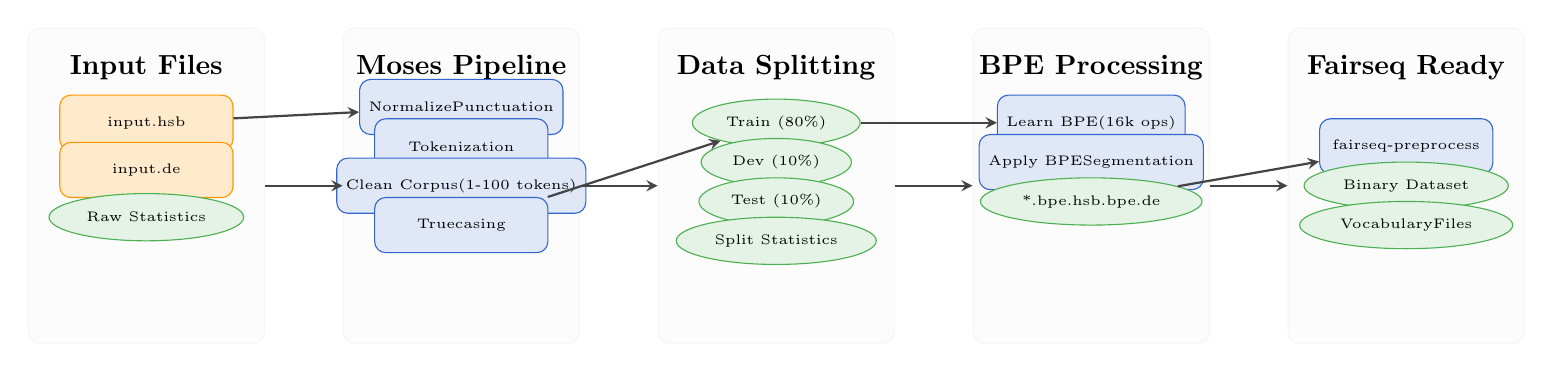
\begin{tikzpicture}[
				node distance=0.8cm and 2.5cm,
				input/.style={rectangle, rounded corners, minimum width=2.2cm, minimum height=0.7cm, text centered, draw=accentorange, fill=accentorange!20, font=\tiny},
				process/.style={rectangle, rounded corners, minimum width=2.2cm, minimum height=0.7cm, text centered, draw=primaryblue, fill=primaryblue!15, font=\tiny},
				output/.style={ellipse, minimum width=1.8cm, minimum height=0.6cm, text centered, draw=secondarygreen, fill=secondarygreen!15, font=\tiny},
				arrow/.style={->,>=stealth,thick,color=darkgray},
				stage/.style={rectangle, rounded corners, minimum width=3cm, minimum height=4cm, draw=lightgray, fill=lightgray!30, font=\scriptsize}
			]

			% Stage 1: Input
			\node (stage1) [stage] at (0,0) {};
			\node at (0,1.5) {\textbf{Input Files}};
			\node (input_hsb) [input] at (0,0.8) {input.hsb};
			\node (input_de) [input] at (0,0.2) {input.de};
			\node (raw_stats) [output] at (0,-0.4) {Raw Statistics};

			% Stage 2: Moses Preprocessing
			\node (stage2) [stage] at (4,0) {};
			\node at (4,1.5) {\textbf{Moses Pipeline}};
			\node (normalize) [process] at (4,1) {Normalize\\Punctuation};
			\node (tokenize) [process] at (4,0.5) {Tokenization};
			\node (clean) [process] at (4,0) {Clean Corpus\\(1-100 tokens)};
			\node (truecaser) [process] at (4,-0.5) {Truecasing};

			% Stage 3: Data Splitting
			\node (stage3) [stage] at (8,0) {};
			\node at (8,1.5) {\textbf{Data Splitting}};
			\node (train_split) [output] at (8,0.8) {Train (80\%)};
			\node (dev_split) [output] at (8,0.3) {Dev (10\%)};
			\node (test_split) [output] at (8,-0.2) {Test (10\%)};
			\node (split_stats) [output] at (8,-0.7) {Split Statistics};

			% Stage 4: BPE Processing
			\node (stage4) [stage] at (12,0) {};
			\node at (12,1.5) {\textbf{BPE Processing}};
			\node (bpe_learn) [process] at (12,0.8) {Learn BPE\\(16k ops)};
			\node (bpe_apply) [process] at (12,0.3) {Apply BPE\\Segmentation};
			\node (bpe_files) [output] at (12,-0.2) {*.bpe.hsb\\*.bpe.de};

			% Stage 5: Final Output
			\node (stage5) [stage] at (16,0) {};
			\node at (16,1.5) {\textbf{Fairseq Ready}};
			\node (fairseq_bin) [process] at (16,0.5) {fairseq-\\preprocess};
			\node (binary_data) [output] at (16,0) {Binary Dataset};
			\node (vocab) [output] at (16,-0.5) {Vocabulary\\Files};

			% Main flow arrows
			\draw [arrow] (stage1.east) -- (stage2.west);
			\draw [arrow] (stage2.east) -- (stage3.west);
			\draw [arrow] (stage3.east) -- (stage4.west);
			\draw [arrow] (stage4.east) -- (stage5.west);

			% Internal arrows (simplified)
			\draw [arrow] (input_hsb) -- (normalize);
			\draw [arrow] (truecaser) -- (train_split);
			\draw [arrow] (train_split) -- (bpe_learn);
			\draw [arrow] (bpe_files) -- (fairseq_bin);

		\end{tikzpicture}
	\end{center}
\end{frame}


\end{document}
